%; whizzy chapter
% -initex iniptex -latex platex -format platex -bibtex jbibtex -fmt fmt
% $B0J>e(B whizzytex $B$r;HMQ$9$k>l9g$N@_Dj!#(B

%     Tokyo Debian Meeting resources
%     Copyright (C) 2011 Junichi Uekawa
%     Copyright (C) 2011 Nobuhiro Iwamatsu

%     Copyright (C) 2012 Koichi Akabe

%     This program is free software; you can redistribute it and/or modify
%     it under the terms of the GNU General Public License as published by
%     the Free Software Foundation; either version 2 of the License, or
%     (at your option) any later version.

%     This program is distributed in the hope that it will be useful,
%     but WITHOUT ANY WARRANTY; without even the implied warranty of
%     MERCHANTABILITY or FITNESS FOR A PARTICULAR PURPOSE.  See the
%     GNU General Public License for more details.

%     You should have received a copy of the GNU General Public License
%     along with this program; if not, write to the Free Software
%     Foundation, Inc., 51 Franklin St, Fifth Floor, Boston, MA  02110-1301 USA

%  preview (shell-command (concat "evince " (replace-regexp-in-string "tex$" "pdf"(buffer-file-name)) "&"))
% $B2hA|%U%!%$%k$r=hM}$9$k$?$a$K$O(Bebb$B$rMxMQ$7$F(Bboundingbox$B$r:n@.!#(B
%(shell-command "cd image201201; ebb *.png")

%%$B$3$3$+$i%X%C%@3+;O!#(B

\documentclass[mingoth,a4paper]{jsarticle}
\usepackage{monthlyreport}

% $BF|IU$rDj5A$9$k!"Kh7nJQ$o$j$^$9!#(B
\newcommand{\debmtgyear}{2012}
\newcommand{\debmtgmonth}{6}
\newcommand{\debmtgdate}{23}
% (+ (* (- 2012 2005) 12) 12 -1) started from zero
\newcommand{\debmtgnumber}{95}


\begin{document}

\dancersection{Gentoo/Prefix on Debian}{$B@DEDD>Bg(B}
\label{sec:your-label}

\subsection{$B$O$8$a$K(B}

$B$$$-$J$j(BGentoo$B$,=P$F$-$F6C$+$l$?$+$b$7$l$^$;$s(B.$B$3$3$G$O(BDebian$B2<$G(B
Gentoo Prefix$B$r%$%s%9%H!<%k$9$kJ}K!$K$D$$$F2r@b$7$^$9(B.

\subsection{Gentoo Prefix}
\subsubsection{Gentoo$B$H$O(B}
Gentoo$B$O(BDebian$B$d(BRPM$B$H0c$C$?%=!<%9%Y!<%9$N%G%#%9%H%j%S%e!<%7%g%s$G$9(B.
ebuild$B$H$$$&%Q%C%1!<%8%S%k%IJ}K!$d(B,$B%Q%C%1!<%8$N0MB84X78$J$I$r5-=R$7$?(B
bash$B%9%/%j%W%HIw$N%U%!%$%k$,(B"$B%+%F%4%j!<(B/$B%Q%C%1!<%8L>(B/$B%Q%C%1!<%8L>(B-$B%Q%C(B
$B%1!<%8%P!<%8%g%s(B.ebuild"$B$H$$$&%U%!%$%kL>$GJ]4I$5$l$F$$$^$9(B. emerge$B$H$$(B
$B$&%3%^%s%I$O(B, $B$3$N(B $B!V(BPortage$B%D%j!<!W$H$$$&%Q%C%1!<%8>pJs%U%!%$%k%D%j!<(B
$B$rFI$s$G;XDj$5$l$?%Q%C%1!<%8$r%S%k%I!&%$%s%9%H!<%k$9$k%Q%C%1!<%84IM}%=%U(B
$B%H$K$J$C$F$$$^$9(B.

\subsubsection{Prefix$B%5%]!<%H(B}

Gentoo$B$b4pK\E*$K$O(BLinux$B>e$N%G%#%9%H%j%S%e!<%7%g%s$G$9$,(B, Debian$B$N(B
Debian GNU/kFreeBSD$B$HF1MM$K(BFreeBSD$B>e$G$N%Q%C%1!<%84IM}$rL\E*$H$7$?(B
Gentoo/FreeBSD$B$J$I$N3+H/$b9T$J$o$l$F$$$^$9(B. $B$=$&$$$C$?(BLinux$B0J30$G$N(B
Gentoo$B$N%5%]!<%H$rAm>N$7$F(B, Gentoo/Alt$B$H8F$s$G$$$^$9(B.
\footnote{http://www.gentoo.org/proj/en/gentoo-alt/} $B$=$N(BGentoo/Alt$B$NCf(B
$B$K(BGentoo Prefix$B$H$$$&$b$N$,$"$j$^$9(B.
\footnote{http://www.gentoo.org/proj/en/gentoo-alt/prefix/index.xml} $B$3(B
$B$l$O(BGentoo$B$N%7%9%F%`$r;H$C$F(B($B4pK\E*$K$O(B)$BB>$N(BOS$B>e$G(B, $BG$0U$N%G%#%l%/%H%j(B
$B$K%Q%C%1!<%8$N%$%s%9%H!<%k$r9T$J$($k$h$&$K$9$k$b$N$G$9(B. $B$?$H$($P(B, Mac
OS X$B>e$GF0$+$7$F(B, MacPorts$B$d(Bhomebrew$B$NBe$o$j$K;H$C$?$j(B, $B$"$k$$$O(B
FreeBSD$B>e$G;H$C$?$j(B, $B$O$?$^$?(BLinux$B>e$G;H$&$3$H$b$b$A$m$s$G$-$^$9(B.

\subsection{Gentoo/Prefix on Debian}

$B$5$F$3$3$+$i$,K\Bj$G(B, $B$3$N(BGentoo/Prefix$B$r(BDebian$B$G;H$C$F$_$^$9(B. $B$*$=$i$/(B
$B$J$s$G$=$s$J$3$H$r!D(B? $B$H;W$o$l$k$+$b$7$l$^$;$s(B. $B0J2<$N$h$&$JE@$,$"$2$i(B
$B$l$k$+$H;W$$$^$9(B.

\begin{itemize}
\item $BHs(Broot$B%f!<%6$G$b9%$-$J$H$3$m$K%$%s%9%H!<%k$G$-$k(B
\item Debian$B$K$J$$%Q%C%1!<%8$r%$%s%9%H!<%k$9$k;~$K3Z$G$-$k(B
\item $B5;=QE*$K3Z$7$$(B?
\end{itemize}

Prefix$B%$%s%9%H!<%k$G$O9%$-$J%G%#%l%/%H%j$K%$%s%9%H!<%k$G$-$k$?$a(B, $B$?$H(B
$B$($P<+J,$N%[!<%`%G%#%l%/%H%j$NCf$J$I$K%$%s%9%H!<%k$9$k$h$&$K$7$F$7$^$((B
$B$P(Broot$B8"8B$,$J$/$H$b%Q%C%1!<%8$r%$%s%9%H!<%k$9$k$3$H$,$G$-$^$9(B. $B$^$?(B,
($B$b$7K|$,0l(B) Debian$B$K$J$$%Q%C%1!<%8$,$"$C$?$H$7$F(B, $B$=$l$,(BGentoo$B$NJ}$K$"(B
$B$l$P(B, $B<+J,$G%S%k%IJ}K!$d0MB8$rD4$Y$k$3$H$J$/(B, Gentoo$B$N%Q%C%1!<%8%7%9%F(B
$B%`$K$*$^$+$;$7$F$7$^$&$3$H$,$G$-$k(B, $B$H$$$&$o$1$G$9(B.

\subsubsection{$B%$%s%9%H!<%k(B}

$B$G$O(B, $B$5$C$=$/(BDebian$B>e$K%$%s%9%H!<%k$7$F$_$^$7$g$&(B. $B$^$:$O%S%k%I$KI,MW(B
$B$J%Q%C%1!<%8$r%$%s%9%H!<%k$7$F$*$-$^$9(B. 

\begin{commandline}
% apt-get install bzip2 build-essential bison libreadline-dev libncurses-dev autoconf xz-utils
\end{commandline}

$B$D$.$K(B, Prefix$B$r%$%s%9%H!<%k$9$k>l=j$r7h$a$F(B,  $BJQ?t(BEPREFIX$B$K@_Dj$7(B, PATH$B$bDL$7$F$*$-$^$9(B.

\begin{commandline}
% export EPREFIX="$HOME/gentoo"
% export PATH="$EPREFIX/usr/bin:$EPREFIX/bin:$EPREFIX/tmp/usr/bin:$EPREFIX/tmp/bin:/usr/bin:/bin:$PATH"
\end{commandline}

Prefix$B$r%$%s%9%H!<%k$9$k$?$a$N%9%/%j%W%H$r<hF@$7(B, $B$=$N%9%/%j%W%H$r;H$C(B
$B$F%Q%C%1!<%84IM}%=%U%H(BPortage$B$H(B, $B%Q%C%1!<%8>pJs$N(BPortage$B%D%j!<$r%$%s%9(B
$B%H!<%k$7$F$$$-$^$9(B. 

\begin{commandline}
% wget http://overlays.gentoo.org/proj/alt/browser/trunk/prefix-overlay/scripts/bootstrap-prefix.sh?format=txt \
  -O bootstrap-prefix.sh
% chmod 755 bootstrap-prefix.sh
% ./bootstrap-prefix.sh $EPREFIX tree
% ./bootstrap-prefix.sh $EPREFIX portage
\end{commandline}

$B$3$N;~E@$G(Bemerge$B%3%^%s%I$,;H$($k$h$&$K$J$j$^$9(B. $B$3$3$+$i$O(Bemerge$B$r;H$C(B
$B$F(B, Prefix$B4D6-$r@0$($F$$$-$^$9(B. $B$3$N$"$?$j$O$"$^$j:#2s$N<gBj$G$O$J$$$N(B
$B$G;D$j$O(BPrefix$B$N%I%-%e%a%s(B
$B%H(B\footnote{http://www.gentoo.org/proj/en/gentoo-alt/prefix/bootstrap-solaris.xml}
$B$r;29M$K$7$F$/$@$5$$(B. \footnote{$B$$$^$N(BDebian$B$@$H(Bmultiarch$B$N1F6A$G$&$^$/(B
  $BF0$+$J$$$H$3$m$b$"$k$+$b$7$l$^$;$s!D(B}

\begin{commandline}

\end{commandline}

\subsection{apt-emerge}

$B$3$3$^$G$G(B, Gentoo/Prefix$B$r2r@b$7$F$-$^$7$?(B. $B$7$+$7(B, $B$3$l$G$O$"$^$j$K(B
Gentoo$B$9$.$^$9$M(B. Gentoo/Prefix$B$NCf$K$b(BDebian$BB&$GF~$C$F$$$k$O$:$N%W%m%0(B
$B%i%`!&%i%$%V%i%j$,%$%s%9%H!<%k$5$l$F$7$^$C$F$J$s$@$+L5BL$J$h$&$J5$$,$7(B
$B$F$7$^$$$^$9(B. $BFC$K(BDebian$B$@$H$5$/$5$/$H%P%$%J%j%Q%C%1!<%8$+$i%$%s%9%H!<(B
$B%k$5$l$F$7$^$&$N$K(B, Gentoo$B$@$H%=!<%9$+$i%S%k%I$5$l$FBT$D$N$b$J$+$J$+Bg(B
$BJQ$J$b$N$G$9(B. $B$J$s$H$+(BDebian$B$K$"$k$b$N$O(BDebian$B$N$b$N$r;H$$$D$D(B, Gentoo
$B$G$O$I$&$7$F$bI,MW$J$b$N$@$1$r%$%s%9%H!<%k$9$k$3$H$O$G$-$J$$$G$7$g$&$+(B.

Gentoo$B$G$O(Betc/portage/profile/package.provided$B%U%!%$%k$K0J2<$N$h$&$K=q(B
$B$/$3$H$G(B, $B$=$N%Q%C%1!<%8$,%$%s%9%H!<%k$5$l$F$$$k$H!V8+Pv$9!W$3$H$,$G$-$^$9(B. 

\begin{commandline}
sys-power/acpi-1.6
sys-power/acpid-2.0.16
sys-process/at-3.1.13
sys-devel/autoconf-2.69
sys-devel/automake-1.11.3
app-shells/bash-4.2
\end{commandline}

Debian$BB&$K$"$k%Q%C%1!<%8$r$3$&$d$C$F(BGentoo$BB&$N%Q%C%1!<%8L>$K%^%C%W$7$F(B,
package.provided$B%U%!%$%k$K=q$/$3$H$G(B, Gentoo$BB&$G0MB8$H$7$F%Q%C%1!<%8$,(B
$B%S%k%I!&%$%s%9%H!<%k$5$l$k$3$H$,$J$/$J$j$^$9(B. $B$3$&$7$F(B

\begin{enumerate}
\item Gentoo$B$N(Bemerge$B$G$N0MB8%Q%C%1!<%8$rGD0.(B
\item Gentoo$B$G$N0MB8%Q%C%1!<%8L>$r(BDebian$B$N%Q%C%1!<%8L>$K%^%C%W(B
\item $B%$%s%9%H!<%k$5$l$?(BDebian$B$N%Q%C%1!<%8L>$r(BGentoo$B$N%Q%C%1!<%8L>$K%^%C%W(B
\item $B%^%C%W$5$l$?%Q%C%1!<%8L>$r(Bpacakge.provided$B$KDI5-(B
\item $B:FEY0MB84X78$r7W;;$7$J$*$7$F(B2$B$KLa$k(B
\item $B$3$l0J>e(BDebian$B$+$i%$%s%9%H!<%k$G$-$J$1$l$P(Bemerge$B$r3+;O(B
\end{enumerate}

$B$H$$$C$?%W%m%;%9$r9T$J$$(B, $B:G>.8B$N%Q%C%1!<%8$@$1$GL\E*$N(BGentoo$B$N%Q%C%1!<(B
$B%8$r%$%s%9%H!<%k$9$k$3$H$,$G$-$^$9(B. $B$3$N;~$K4N$H$J$k$N$,(B, $B!V(BGentoo$B$G$N(B
  $B0MB8%Q%C%1!<%8$NGD0.!W$H!V(BGentoo$B$H(BDebian$B$H$N%Q%C%1!<%8$NAj8_%^%C%W$r(B
  $B$I$&$9$k$N$+!W$NFsE@$G$9(B.

\subsubsection{Gentoo$B$G$N0MB8%Q%C%1!<%8(B}

emerge$B$KBP$7$F0J2<$N%*%W%7%g%s$r$D$1$F=PNO$r2r@O$7$^$9(B.

\begin{itemize}
\item -p (--pretend): $B%$%s%9%H!<%k$r<B9T$;$:%$%s%9%H!<%k%Q%C%1!<%80lMw$@$1$r=PNO$7$^$9(B
\item -q (--quiet): $BL5BL$J>pJs$r=PNO$7$J$$$h$&$K$7$^$9(B
\item -t (--tree): $B%$%s%9%H!<%k$9$k%Q%C%1!<%8$r0MB84X78$N%D%j!<>u$K=PNO$7$^$9(B
\end{itemize}

-t$B$,0lHV=EMW$J$H$3$m$G$9(B. $B$3$l$r;XDj$9$k$3$H$G$3$N$h$&$K%D%j!<>u$K=PNO$5$l$^$9(B

\begin{commandline}
%  emerge -pqt --quiet-repo-display chromium
[ebuild  N    ] www-client/chromium-20.0.1132.21 
...
[nomerge      ] www-client/chromium-20.0.1132.21 
[ebuild  N    ]  dev-libs/nss-3.13.4 
[ebuild  N    ]   dev-libs/nspr-4.9 
[ebuild  N    ]    sys-devel/autoconf-2.13 
[ebuild  N    ]     sys-devel/autoconf-wrapper-12 
[ebuild  N    ]   dev-db/sqlite-3.7.12.1 
...
\end{commandline}

$B$3$N%D%j!<$N@u$$$H$3$m$+$i(BDebian$B$N%Q%C%1!<%8$X$H%^%C%W$7$F$$$-$^$9(B. $B@u(B
$B$$$H$3$m$+$i%^%C%W$7$F$$$/$3$H$G(B, $B$G$-$k$@$1B?$/$N0MB82r7h$r(BDebian$BB&$K(B
$B$*$^$+$;$7$^$9(B. $B$D$^$j(B, $B$?$H$($P$3$3$G(B dev-libs/nspr$B$r(BDebian$BB&$G%$%s%9(B
$B%H!<%k$9$k$3$H$K@.8y$9$l$P$3$N%D%j!<$r(B

\begin{commandline}
[ebuild  N    ] www-client/chromium-20.0.1132.21 
...
[nomerge      ] www-client/chromium-20.0.1132.21 
[ebuild  N    ]  dev-libs/nss-3.13.4 
[ebuild  N    ]   dev-db/sqlite-3.7.12.1 
...
\end{commandline}

$B$3$3$^$G0l5$$K=L>.$9$k$3$H$,$G$-$k$H$$$&$o$1$G$9(B. 

\subsubsection{Gentoo$B$+$i(BDebian$B$X$N%^%C%W(B}

Gentoo$B$N%Q%C%1!<%8L>$+$i(BDebian$B$N%Q%C%1!<%8L>$X$N%^%C%T%s%0$r9T$J$$$^$9(B.
Gentoo$B$N%Q%C%1!<%8L>$K$O%+%F%4%j$,$D$$$F$$$^$9$,(B, Debian$B$NJ}$K$O$=$l$,(B
$B$J$$$N$G(B, $B$H$j$"$($:30$7$F$7$^$$$^$9(B. $B$=$7$F(B, $B0J2<$N=gHV$GC5:w$r$+$1$^$9(B. 

\begin{itemize}
\item lib$B%Q%C%1!<%8L>(B-dev
\item $B%Q%C%1!<%8L>(B-dev
\item $B%Q%C%1!<%8L>(B
\end{itemize}

Gentoo$B$N%Q%C%1!<%8$G$O0lHL$K(BDebian$B$N(B*-dev$B$KF~$k$h$&$J$b$N$,%$%s%9%H!<%k(B
$B$5$l$F$$$k$N$G(B, *-dev$B$rM%@h$7$F%$%s%9%H!<%k$9$k$h$&$K$7$F$$$^$9(B. 

$B$^$?(B, dev-ruby$B%+%F%4%j$N$b$N$K$O(Bruby-$B$r%Q%C%1!<%8L>$K$D$1$k$J$I$N9)IW$r(B
$B$7$?$j(B, $B$I$&$7$F$b$3$l$G%^%C%W$G$-$J$$$b$N$OL@<(E*$K%^%C%T%s%0$r=q$/$J(B
$B$I$NBP=h$b$7$F$$$^$9(B.

\subsubsection{Debian$B$+$i(BGentoo$B$X$N%^%C%W(B}

$B$3$&$7$F(BDebian$B$X$H%Q%C%1!<%8$r%$%s%9%H!<%k$G$-$?$i(B, $B%$%s%9%H!<%k$G$-$?(B
$B%Q%C%1!<%8$N%P!<%8%g%s$r<hF@$7$F(BGentoo$B$N%Q%C%1!<%8L>$X$N%^%C%W$r$7$F$$(B
$B$-$^$9(B. $B$3$l$OC1=c$K(Bdpkg -l ...$B$N7k2L$r;H$&$@$1$G$9$M(B. $B8=>u(BDebian$B$N2>A[(B
$B%Q%C%1!<%8$+$iA*Br$5$l$k<B:]$N%Q%C%1!<%8$N%P!<%8%g%s$r$H$l$:(B, $B$&$^$/%^%C(B
$B%W$G$-$F$$$^$;$s!D(B.

\subsubsection{$B<B9T%5%s%W%k(B}

$B$3$l$i$N%"%$%G%"$r<BAu$7$?$N$,(Bapt-emerge$B%9%/%j%W%H$K$J$j$^$9(B. $B$3$N%9%/(B
$B%j%W%H$O4pK\E*$K>e5-$N(Bemerge$B$,;H$($k$h$&$K$J$C$?CJ3,$G;H$($k$h$&$K$J$C(B
$B$F$$$^$9$,(B, $B0lIt$N%Q%C%1!<%8$O(BGentoo$B$N%3%"ItJ,$KBg$-$/?)$$$3$s$G$$$k$N(B
$B$G$=$l$i$O(BGentoo$B$GF~$l$F$*$+$J$$$H$$$1$^$;$s(B. $B$^$?(B, Debian$B$N(Bmultiarch$B$K(B
$BBP1~$9$k$h$&$K(BCFLAGS/LDFLAGS$B$rD4@0$7$^$9(B.
 
\begin{commandline}
% vi $EPREFIX/etc/make.conf
CFLAGS="-O2 -I/usr/include/x86_64-linux-gnu"
LDFLAGS="${LDFLAGS} -L/usr/lib/x86_64-linux-gnu"
% FEATURES="-collision-protect" emerge -avg1 --nodeps bash eselect eselect-python python portage libffi
\end{commandline}

$B$3$l$G(Bapt-emerge$B$,F0$/$h$&$K$J$k$O$:$G$9(B. apt-emerge$B$rF0$+$9$H<+F0E*$KI,MW$J%Q%C%1!<%8$r(Bapt-get$B$KEO$7(B, $B2DG=$J8B$j$N0MB8$r2r7h$7$F$+$i(B, emerge$B$K=hM}$rEO$7$^$9(B.

$BNc$H$7$F(BTwitter$B%/%i%$%"%s%H(B
mikutter\footnote{http://mikutter.hachune.net}$B$r(Bapt-emerge$B$G%$%s%9%H!<(B
$B%k$7$F$_$^$7$g$&(B. $B$3$l$O(BRuby$B$H(BRuby/Gtk2$B$J$I$r;H$C$?%Q%C%1!<%8$J$N$G(B, $BIa(B
$BDL$K(Bemerge$B$9$k$@$1$G$"$l$P(B, gtk$B$J$IBgNL$K%S%k%I$5$l$k$O$:$G$9(B
$B$,!D!D(Bapt-emerge mikutter$B8e$K(BGentoo$BB&$K$J$K$,%$%s%9%H!<%k$5$l$F$$$k$+$r(B
$B%j%9%H%"%C%W$7$F$_$^$7$g$&(B($B2>A[%Q%C%1!<%8$O=|$$$F$"$j$^$9(B)

\begin{commandline}
% eix -I -c |grep -v virtual
[I] app-admin/eselect (1.3.1@06/03/2012): Gentoo's multi-purpose configuration and management tool
[I] app-admin/eselect-python (20111108@06/03/2012): Eselect module for management of multiple Python versions
[I] app-admin/python-updater (0.10-r2@06/04/2012): Script used to reinstall Python packages after changing of active Python versions
[U] app-shells/bash (4.2_p28@06/03/2012 -> 4.2_p29): The standard GNU Bourne again shell
[I] app-shells/push (1.5@06/04/2012): A POSIX shell function to treat a variable like an array, quoting args.
[I] dev-lang/python (2.7.3-r2(2.7)@06/04/2012): Python is an interpreted, interactive, object-oriented programming language.
[I] dev-libs/libffi (3.0.11@06/04/2012): a portable, high level programming interface to various calling conventions.
[I] net-misc/mikutter (9999@06/04/2012): mikutter is simple, powerful and moeful twitter client
[I] sys-apps/baselayout-prefix (1.12.14@06/04/2012): Baselayout for Gentoo Prefix installs
[I] sys-apps/portage (2.2.01.20430@06/04/2012): Prefix branch of the Portage Package Manager, used in Gentoo Prefix
[I] sys-apps/tcp-wrappers (7.6.22@06/04/2012): TCP Wrappers
[I] sys-devel/gnuconfig (20120116@06/04/2012): Updated config.sub and config.guess file from GNU
\end{commandline}

$B$4Mw$N$h$&$K(B10$B8DDxEY$7$+(BGentoo$BB&$K$O%$%s%9%H!<%k$5$l$F$$$^$;$s$,(B,
mikutter-9999 (SVN trunk$B$N%P!<%8%g%s(B)$B$,$7$C$+$j$H%$%s%9%H!<%k$5$l$F$$$^$9(B.

\subsection{$B$3$l$+$i(B}

apt-emerge$B$N%9%/%j%W%H$O$^$@%3%s%;%W%H$,<BAu$5$l$?$@$1$G(B, $B$$$m$s$JItJ,(B
$B$,(Bad-hoc$B$K$J$C$F$$$^$9(B. $B$h$j(BDebian$B$N%Q%C%1!<%8L>$H(BGentoo$B$N%Q%C%1!<%8L>(B
$B$H$N%^%C%T%s%0$N?dB,$r8-$/$7$?$j(B, $BI,MW$J8GDj%^%C%W%G!<%?$r3H=<$7(B,
Debian$B$N(Bvirtual$B%Q%C%1!<%8$r$&$^$/=hM}$7$?$j$9$k$J$I(B, $B$h$j;H$$$d$9$$%S%k(B
$B%I%7%9%F%`$r:n$l$l$P$H;W$$$^$9(B. $B<+J,<+?H(BDebian$B$K?<$/CN<1$r;}$C$F$$$k$o(B
$B$1$G$O$J$$$N$G(B, $B$b$7$+$9$k$H$b$C$H8zN($N$h$$<BAu$b$"$k$+$b$7$l$^$;$s!D(B.
$B$b$76=L#$r;}$C$F$$$?$@$1$l$P(B, $B3+H/;22C!&%"%I%P%$%9$7$F$$$?$@$1$^$7$?$i(B
$B9,$$$G$9(B. 

\dancersection{IPython notebook$B$H$=$N<~JU(B}{$BK\>190E5(B}
\label{sec:ipython-notebook}

\subsection{$B$O$8$a$K(B}

$B:G6a(Bipython$B$N(Bqtconsole$B$G%3%s%=!<%k>e$K%0%i%U$rIA2h$7$F$$$k%9%/%j!<%s%7%g%C%H$r8+$k5!2q$,$"$j!"(B
$B$A$g$C$H$+$C$3$$$$$+$J$H%m%/$K;H$C$?$3$H$,$J$$(BPython$B$r;H$$;O$a$^$7$?!#(B
$B:#2s$O(Bipython qtconsole$B$r;HMQ$7$?%0%i%U$NIA2h$+$i!"(B
Mathmatica notebooks$B$N$h$&$J(BWeb$B%Y!<%9$N?t<0=hM}%7%9%F%`(Bipython notebook$B$r(BPython$B=i?4<T$N;kE@$G>R2p$7$F$_$?$$$H;W$$$^$9!#(B

\subsection{IPython}

ipython$B$O(BFernando Perez$B;a$K$h$C$F:n@.$5$l$?(BPython$B$N%$%s%?%i%/%F%#%V%7%'%k$G!"(B
$B8=:_$N:G?7%j%j!<%9%P!<%8%g%s$O(B0.12.1$B$G$9!#(B
Python$B$O$=$l<+BN$G%$%s%?%i%/%F%#%V%7%'%k$N5!G=$r;}$C$F$$$^$9$,!"(B
ipython$B$O(BPython$B%7%'%k$HHf3S$7$F<!$NFCD'$r;}$C$F$$$^$9!#(B

\begin{itemize}
 \item terminal$B$G$N;HMQ$K2C$((BQt$BEy$rMQ$$$?%0%i%U%#%+%k$J%3%s%=!<%k$,;HMQ2DG=(B
 \item $B%3!<%IJd40(B
 \item $B%7%s%?%C%/%9%O%$%i%$%H(B
 \item $BJBNs%3%s%T%e!<%F%#%s%0$,2DG=(B
 \item Web$B%Y!<%9$N(Bnotebook(ipython 0.12$B$+$i(B)
\end{itemize}

Python$B%7%'%k$H(Bipython$B$O<!$N?^$N$h$&$K!"(B
$B%W%m%s%W%HEy$K0c$$$,$"$j$^$9!#(B

\begin{figure*}[b]
  \begin{tabular}{cc}
    \begin{minipage}[b]{0.5\textwidth}
      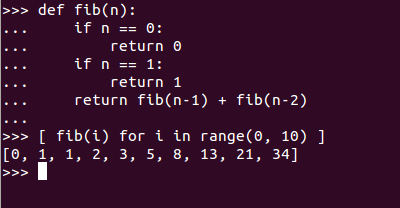
\includegraphics[width=1.0\hsize]{images/ipython-pythonshell.png}
      \label{pythonshell}
    \end{minipage}
    \begin{minipage}[b]{0.5\textwidth}
      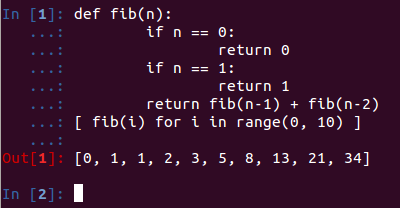
\includegraphics[width=1.0\hsize]{images/ipython-terminal.png}
      \label{ipython}
    \end{minipage}
  \end{tabular}
  \caption{python$B%7%'%k$H(Bipython$B$N0c$$(B}
\end{figure*}

\subsection{IPython qtconsole}

ipythopn$B$K(Bqtconsole$B%*%W%7%g%s$r;XDj$7$F<B9T$9$k$3$H$K$h$j!"(B
GUI$B4D6-$G$N(Bipython$B$,5/F0$7$^$9!#(B
$B$^$?$3$N4D6-$G(B--pylab inline$B$r;XDj$7$F5/F0$9$k$3$H$G!"(B
$B%3%s%=!<%kFb$K%0%i%U$rI=<($5$;$k$3$H$,2DG=$H$J$j$^$9!#(B

\begin{commandline}
$ ipython qtconsole --pylab matplotlib
\end{commandline}

$B$3$N4D6-$G$OA0=R$N%0%i%UI=<($K2C$(!"(B
$BJ#?t9T$r$^$H$a$F07$&%3%^%s%I$NMzNr$J$I$,;HMQ$G$-$^$9!#(B
$B%0%i%U$rIA2h$9$k$H<!$N$h$&$KI=<($5$l$^$9!#(B

\begin{figure}[ht]
  \begin{center}
    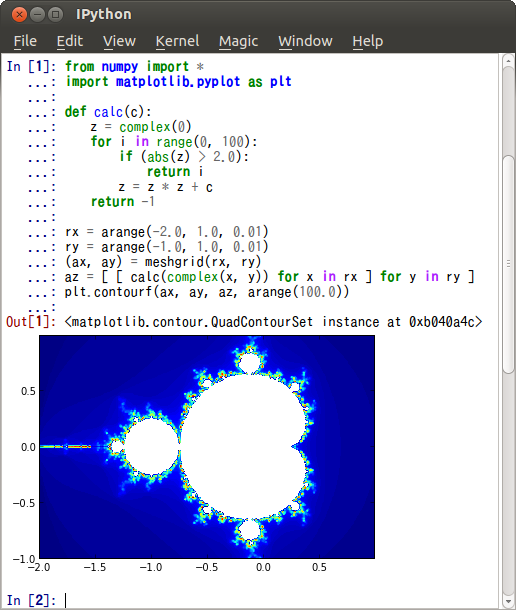
\includegraphics[width=0.6\hsize]{images/ipython-mandelbrotset.png}
  \end{center}
  \caption{qtconsole$B$G%^%s%G%k%V%m=89g(B}
  \label{fig:ipython-qtconsole}
\end{figure}

testing$B$G$N(Bipython qtconsole$B$*$h$S(Bmatplotlib$B$O<!$N%3%^%s%I$G%$%s%9%H!<%k=PMh$^$9!#(B

\begin{commandline}
$ sudo aptitude install ipython-qtconsole python-matplotlib
\end{commandline}

$B$^$?(Bsqueeze$B$O(Bbackports$B$r;HMQ$7$F%$%s%9%H!<%k$r9T$$$^$7$?!#(B
$B$^$:(B/etc/apt/sources.list$B$K<!$N9T$rDI2C$7!"(B

\begin{commandline}
deb http://backports.debian.org/debian-backports squeeze-backports main
\end{commandline}

aptitude update \&\& aptitude upgrade$B$r<B9T$7$?8e!"(B
$B<!$N%3%^%s%I$G%$%s%9%H!<%k$7$^$9!#(B

\begin{commandline}
$ sudo aptitude install python-setuptools python2.6-dev ncurses-dev libzmq-dev python-pygments python-matplotlib pyqt4-dev-tools
\end{commandline}

$B%Q%C%1!<%8$N%$%s%9%H!<%k8e!"(B
python$B$N(Beasy\_install$B%3%^%s%I$r;HMQ$7$F(Bipython$B$r%$%s%9%H!<%k$7$^$9!#(B

\begin{commandline}
$ sudo easy_install readline pyzmq ipython
\end{commandline}

\subsection{IPython notebook}

ipython notebook$B$O(BWeb$B%Y!<%9$N?t<0=hM}%7%9%F%`$G!"(B
$B<!$N5!G=$rHw$($F$$$^$9!#(B

\begin{itemize}
 \item Python$B%3!<%I$N<B9T$H7k2L$NI=<((B
 \item Markdown$B$K$h$k%^!<%/%"%C%W2DG=$J%N!<%H(B
 \item MathJax$B$K$h$k(B \TeX $B7A<0$G$N?t<0$N5-=R(B
\end{itemize}

\begin{figure}[ht]
  \begin{center}
    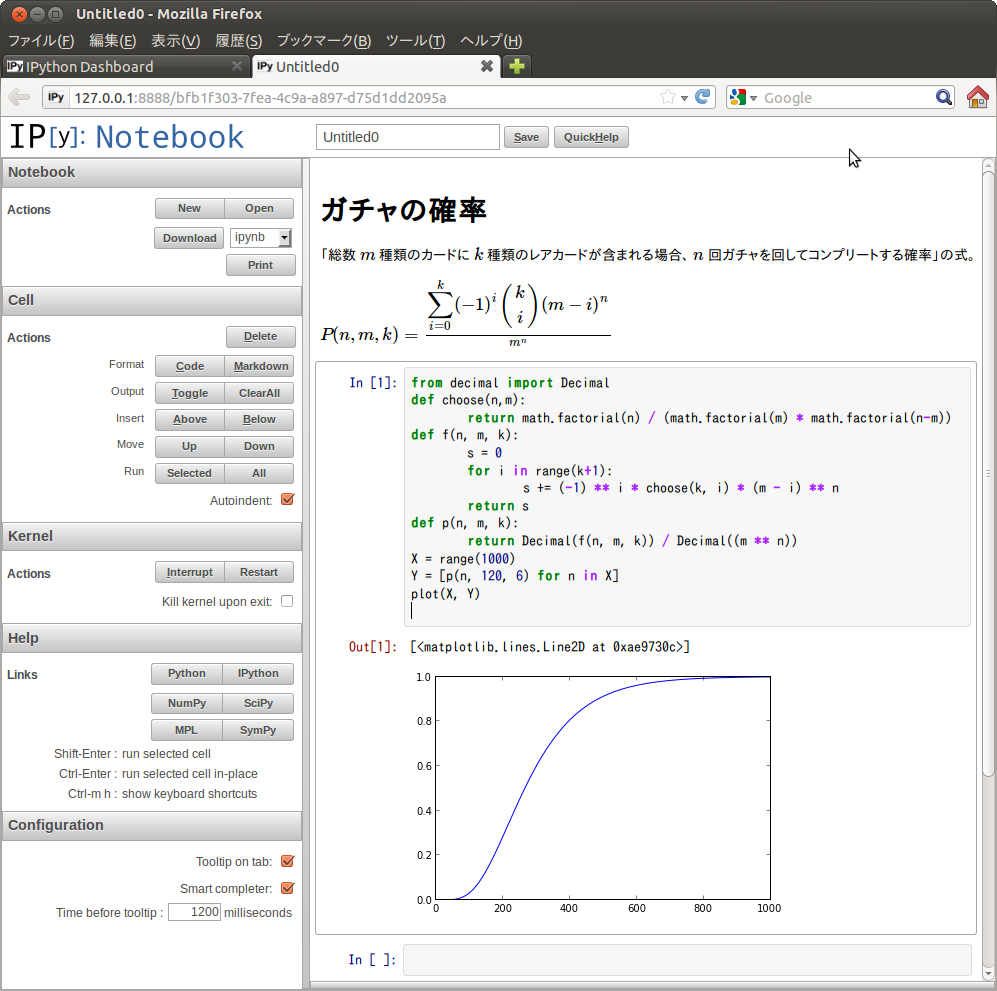
\includegraphics[width=0.80\hsize]{images/ipython-gacha.png}
  \end{center}
  \caption{ipython notebook$B$N;HMQNc(B}
  \label{fig:ipython-gacha}
\end{figure}

testing$B$K$O<!$N%3%^%s%I$G%$%s%9%H!<%k2DG=$G$9!#(B

\begin{commandline}
$ sudo aptitude install ipython-notebook python-matplotlib python-tornado
\end{commandline}

squeeze$B$O(Bqtconsole$B$HF1MM$K(Bbackports$B$r;HMQ$7$^$9!#(B
$B$3$3$G$O(Bsqueeze$B$N(Biceweasel$B$,8E$$$?$a$3$A$i$b(Bapt line$B$KDI2C$7$F$$$^$9!#(B

\begin{commandline}
deb http://backports.debian.org/debian-backports squeeze-backports main
deb http://mozilla.debian.net/ squeeze-backports iceweasel-release
\end{commandline}

aptitude update \&\& aptitude upgrade$B$r<B9T$7$?8e!"(B
$B%$%s%9%H!<%k$O<!$N%3%^%s%I$G9T$$$^$7$?!#(B

\begin{commandline}
$ sudo aptitude install python-setuptools python2.6-dev ncurses-dev libzmq-dev python-pygments python-matplotlib
\end{commandline}

$B%Q%C%1!<%8$r%$%s%9%H!<%k$7$?8e!"(B
python$B$N(Beasy\_install$B%3%^%s%I$r;HMQ$7$F(Bipython$B$r%$%s%9%H!<%k$7$^$9!#(B

\begin{commandline}
$ sudo easy_install readline pyzmq ipython tornado
\end{commandline}

$B$^$?$3$N$^$^$G$O(BMathJax$B$,(BCDN$B$r;X$7$F$$$k$N$G!"(B
python$B$r4IM}<T8"8B$G<B9T$7%m!<%+%k$K%$%s%9%H!<%k$7$^$9!#(B

\begin{commandline}
from IPython.external.mathjax import install_mathjax
install_mathjax()
\end{commandline}

squeeze$B$N%&%'%V%V%i%&%6$O$I$l$b8E$/!"(B
Web Socket$B$NLdBj$+$i(Bnotebook$B$G$O;H$($^$;$s!#(B
$B$=$3$G:G?7HG$N(Biceweasel$B$rF3F~$7$^$9!#(B
ipython notebook$B$O5/F0;~$K%G%U%)%k%H%V%i%&%6$r5/F0$9$k$?$a!"(B
$BF3F~8e$O(Biceweasel$B$r%G%U%)%k%H%V%i%&%6$K;XDj$7$F$/$@$5$$!#(B

\begin{commandline}
$ sudo aptitude install -t squeeze-backports iceweasel
\end{commandline}

ipython notebook$B$O<!$N%3%^%s%I$G5/F0$7$^$9!#(B

\begin{commandline}
$ ipython notebook --pylab inline
\end{commandline}

$BB>$N%^%7%s$+$i@\B3$r9T$&>l9g!"(B
$B%V%i%&%6$r5/F0$5$;$J$$$?$a%*%W%7%g%s(B''--no-browser''$B$r!"(B
$B%"%/%;%95v2D$rM?$($k$?$a(Bnotebook$B$r5/F0$5$;$k%^%7%s$N(Bip$B%"%I%l%9$r%*%W%7%g%s(B''--ip''$B$G;XDj$7$^$9!#(B

\begin{commandline}
$ ipython notebook --pylab inline --no-browser --ip 192.168.1.40
\end{commandline}

$B=i2s5/F0;~$K$O<!$N$h$&$J2hLL$,I=<($5$l$^$9!#(B

\begin{figure}[ht]
  \begin{center}
    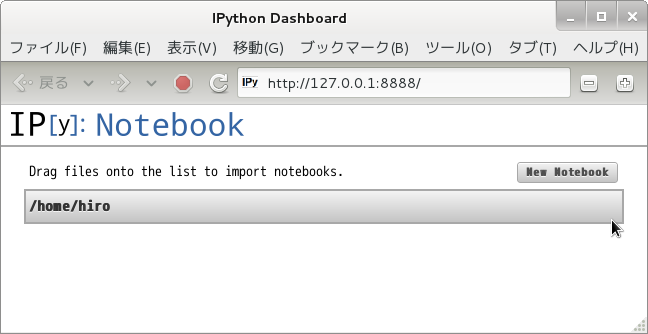
\includegraphics[width=0.67\hsize]{images/ipython-notebook.png}
  \end{center}
  \caption{ipython notebook$B$r5/F0$7$?D>8e(B}
  \label{fig:ipython-notebook}
\end{figure}

$B!V(BNew Notebook$B!W%\%?%s$r%/%j%C%/$9$k$3$H$G?75,%N!<%H%V%C%/$,:n@.$5$l!"(B
$B6u$N%N!<%H%V%C%/$,%V%i%&%6$KI=<($5$l$^$9!#(B
Markdown$B$H(BPython$B$N(BCell$B$O(BCtrl-m m$B$*$h$S(BCtrl-m c$B$G@Z$jBX$($k$3$H$,$G$-!"(B
$B$=$NB>%3%^%s%I$N>\:Y$O(BCtrl-m h$B$GI=<($5$l$^$9!#(B

$B:n@.$5$l$?%N!<%H%V%C%/$OI=<($5$l$F$$$k%G%#%l%/%H%j(B($B$3$3$G$O(B/home/hiro/)$B$K(B''$<$ $B%N!<%H%V%C%/$N%?%$%H%k(B$>$.ipynb''$B$H$$$&%U%!%$%kL>$GJ]B8$5$l$^$9!#(B
$B$3$N%U%!%$%k$NCf?H$O(BJSON$B7A<0$H$J$C$F$$$^$9!#(B

\subsection{$B:G8e$K(B}

$B:#2s$O(Bipython qtconsole$B$*$h$S(Bnotebook$B$r(BDebian$B$G;HMQ$9$kJ}K!$r>R2p$7$^$7$?!#(B
Ubuntu 12.04$B$G$O$I$A$i$b%Q%C%1!<%8$H$7$FDs6!$5$l$F$$$k$?$a!"(B
wheezy$B$G$O%$%s%9%H!<%k:n6H$,4JC1$K$J$k$H;W$o$l$^$9!#(B
$B$3$l$r5!2q$K(Bipython$B$r3hMQ$7$F$$$?$@$1$l$P9,$$$G$9!#(B

\dancersection{Linux-PAM$B$N@_Dj$K$D$$$F(B}{$B@>;3OB9-(B}
\label{sec-1}
\subsection{Introduction}
\label{sec-1-1}
\subsubsection{PAM $B$H$O2?$+(B?}
\label{sec-1-1-1}

Linux-PAM (Pluggable Authentication Modules for Linux) $B$H$O!"%"%W%j%1!<%7%g%s$,%f!<%6!<$r$I$&G'>Z$9$k$+$r%m!<%+%k%7%9%F%`$N4IM}<T$,@_Dj$G$-$k$h$&$K$9$k$?$a$N6&M-%i%$%V%i%j0l<0$G$9!#(B

PAM $B$N$*$+$2$G!"%"%W%j%1!<%7%g%s$r%3%s%Q%$%k$7$J$*$5$J$/$F$b!"G'>ZJ}K!$rJQ99$7$?$j!"8"8B$NIUM?$N;EJ}$rJQ99$7$?$j$G$-$k$h$&$K$J$C$F$$$^$9!#(B
\subsubsection{NSS $B$H$O2?$+(B?}
\label{sec-1-1-2}

PAM $B$H4X78$N?<$$%i%$%V%i%j$H$7$F(B NSS (Name Service Switch) $B$,$"$j$^$9!#(B
NSS $B$O%f!<%6!<L>$H%f!<%6!<(B ID $B$H$NJQ49$r$7$?$j!"%[%9%HL>$H(B IP $B%"%I%l%9$H$NJQ49$r$7$?$j$9$k$H$-$K;H$o$l$^$9!#(B
\subsubsection{PAM $B$H(B NSS $B$H$N0c$$(B}
\label{sec-1-1-3}

PAM $B$OG'>ZItJ,$N$_$J$N$G!"4pK\E*$K$O%m%0%$%s$d%m%0%"%&%H$N$H$-$H%Q%9%o!<%IJQ99$K4X78$7$^$9!#(B ($B87L)$K$O%"%W%j%1!<%7%g%s<!Bh$G$9!#(B)

$B%m%0%$%sCf$K(B \verb~id~ $B%3%^%s%I$GI=<($5$l$k%f!<%6!<(BID$B$H%f!<%6!<L>$NBP1~(B \footnote{$B%0%k!<%W(BID$B$H%0%k!<%WL>$bF1MM$G$9!#(B } $B$d(B \verb~ls -l~ $B$G%U%!%$%k%7%9%F%`$K5-O?$5$l$F$$$k%f!<%6!<(BID$B$+$i%f!<%6!<L>$X$NJQ49(B \footnote{$B%U%!%$%k%7%9%F%`$K$O=jM-<T$O%f!<%6!<(BID$B$G5-O?$5$l$F$$$^$9!#$=$N$?$a!"$?$H$($P%f!<%6!<$r:o=|$7$FB8:_$7$J$$%f!<%6!<$N%U%!%$%k$,$"$k>l9g$K$O!"%f!<%6!<L>$X$NJQ49$,=PMh$J$$$N$G?t;z$GI=<($5$l$^$9!#(B } $B$J$I$O(B \verb~/etc/nsswitch.conf~ $B$G@_Dj$9$k(B NSS $B$N5!G=$K$J$j$^$9!#(B
\subsubsection{PAM $B$N@_Dj(B}
\label{sec-1-1-4}

PAM $B$O@_Dj%U%!%$%k$K<B9T$7$?$$%b%8%e!<%k$rJB$Y$F$*$$$F!"$=$l$r=gHV$K<B9T$7$F$$$/$h$&$J$b$N$@$H;W$($PNI$$$G$7$g$&!#(B

$B$?$H$($P(B
\begin{itemize}
\item \verb~/etc/passwd~ $B$J$I$N%m!<%+%k%U%!%$%k$G$NG'>Z(B
\begin{itemize}
\item $B@.8y$9$l$PG'>Z@.8y$r%"%W%j%1!<%7%g%s$KJV$9(B
\item $B<:GT$9$l$P<!$X(B
\end{itemize}
\item LDAP $B$G$NG'>Z(B
\begin{itemize}
\item $B@.8y$9$l$PG'>Z@.8y$r%"%W%j%1!<%7%g%s$KJV$9(B
\item $B<:GT$9$l$P<!$X(B
\end{itemize}
\item $B<!$,$J$$$N$GG'>Z<:GT$r%"%W%j%1!<%7%g%s$KJV$9(B
\end{itemize}
$B$H$$$&F0:n$r$7$^$9!#(B
\subsection{$B%U%!%$%kG[CV(B}
\label{sec-1-2}
\subsubsection{$B@_Dj%U%!%$%k(B}
\label{sec-1-2-1}

\verb~/etc/pam.d/~ $B$N2<$K%"%W%j%1!<%7%g%s$4$H$N@_Dj%U%!%$%k$,$"$j$^$9!#(B
$B0J2<$O$=$NNc$G$9!#(B


\begin{commandline}
% ls /etc/pam.d
atd       chsh            common-password                cron      other   su
chfn      common-account  common-session                 login     passwd  sudo
chpasswd  common-auth     common-session-noninteractive  newusers  sshd
\end{commandline}

\begin{itemize}
\item $B$I$N@_Dj%U%!%$%k$,$I$N%"%W%j%1!<%7%g%s$N$b$N$J$N$+$O%U%!%$%kL>$+$i?dB,$G$-$^$9!#(B
\item $B$J$$>l9g$O(B \verb~other~ $B$,;H$o$l$^$9!#(B
\item $B$=$l$>$l$NCf$+$i(B \verb~@include~ $B$G(B \verb~common-*~ $B$G6&DL$N@_Dj$r;H$&$h$&$K$J$C$F$$$^$9!#(B
\end{itemize}

\verb~/etc/pam.d/~ $B$,$J$$>l9g$O(B \verb~/etc/pam.conf~ $B$,;H$o$l$k$H(B \verb~/etc/pam.conf~ $B$NCf$N%3%a%s%H$K=q$$$F$"$j$^$9$,!"Nr;KE*$J$b$N$G:G6a$N(B Linux $B$G$O;H$o$l$F$$$^$;$s!#(B
\subsubsection{$B%b%8%e!<%k(B}
\label{sec-1-2-2}

$B0J2<$O(B PAM $B%b%8%e!<%k$NNc$G$9!#(B


\begin{commandline}
% ls /lib/x86_64-linux-gnu/security
pam_access.so     pam_keyinit.so    pam_nologin.so     pam_tally.so
pam_debug.so      pam_lastlog.so    pam_permit.so      pam_tally2.so
pam_deny.so       pam_ldap.so       pam_pwhistory.so   pam_time.so
pam_echo.so       pam_limits.so     pam_rhosts.so      pam_timestamp.so
pam_env.so        pam_listfile.so   pam_rootok.so      pam_umask.so
pam_exec.so       pam_localuser.so  pam_securetty.so   pam_unix.so
pam_faildelay.so  pam_loginuid.so   pam_selinux.so     pam_userdb.so
pam_filter.so     pam_mail.so       pam_sepermit.so    pam_warn.so
pam_ftp.so        pam_mkhomedir.so  pam_shells.so      pam_wheel.so
pam_group.so      pam_motd.so       pam_stress.so      pam_xauth.so
pam_issue.so      pam_namespace.so  pam_succeed_if.so
\end{commandline}

\begin{itemize}
\item $B@_Dj%U%!%$%k$K=q$+$l$k(B \verb~pam_unix.so~ $B$J$I$O(B \verb~dlopen(3)~ $B$GF0E*$KFI$_9~$^$l$^$9!#(B
\item $B$=$N$?$a(B PAM $B$NG'>Z$r;H$C$F$$$k%W%m%0%i%`$rF~$l$?(B chroot $B4D6-$r:n$k$H$-$K$O5$$r$D$1$kI,MW$,$"$j$^$9!#(B
\item \verb~squeeze~ $B$^$G$O(B \verb~/lib/security/~ $B$d(B \verb~/lib64/security/~ $B$K$"$j$^$9!#(B
\item \verb~multiarch~ $BBP1~$G:G6a$O(B \verb~/lib/x86_64-linux-gnu/security/~ $B$J$I$N(B \verb~/lib/<triplet>/security/~ $B$K$"$j$^$9!#(B
  $B>e5-$NNc$O(B wheezy (testing) $B$J$N$G(B \verb~/lib/security/~ $B$G$O$J$/(B
  \verb~/lib/x86_64-linux-gnu/security/~ $B$K$J$C$F$$$^$9!#(B
\end{itemize}
\subsection{$B@_Dj%U%!%$%k$N=q<0(B}
\label{sec-1-3}

$B@_Dj%U%!%$%k$NNc$r:\$;$F$*$-$^$9!#(B($B0lIt>JN,(B)

\begin{commandline}
% egrep '^[^#]' /etc/pam.d/cron
@include common-auth
session       required   pam_env.so
session       required   pam_env.so envfile=/etc/default/locale
@include common-account
@include common-session-noninteractive
session    required   pam_limits.so
\end{commandline}

\begin{itemize}
\item $B@_Dj%U%!%$%k$K$O0J2<$N9`L\$r;XDj$7$^$9!#>\:Y$O8e=R$7$^$9!#(B
\begin{description}
\item[\verb~service~] $B%"%W%j%1!<%7%g%s$KBP1~$9$kL>A0(B
\item[\verb~type~] PAM $B$NJ,N`(B
\item[\verb~control~] $BF0:n;XDj(B
\item[\verb~modules-path~] PAM $B%b%8%e!<%k$X$N%Q%9(B
\item[\verb~module-arguments~] PAM $B%b%8%e!<%k$N0z?t(B
\end{description}
\item \verb~#~ $B$+$i9TKv$^$G$O%3%a%s%H$K$J$j$^$9!#(B
\item \verb~\~ $B$,2~9T(B (\verb~<LF>~) $B$ND>A0$K$"$k$H7QB39T$K$J$j$^$9!#(B
\item \verb~/etc/pam.conf~ $B$G$O!V(B \verb~service type control module-path module-arguments~ $B!W$H$$$&=q<0$G@_Dj$7$^$9!#(B( \verb~service~, \verb~type~, \verb~control~ $B$NBgJ8;z>.J8;z$OL5;k$5$l$^$9!#(B)
\item \verb~/etc/pam.d/~ $B$G$O(B \verb~service~ $B$,%U%!%$%kL>(B ($BI,$:>.J8;z(B) $B$K$J$j$^$9!#(B
\item $B;D$j$N!V(B \verb~type control module-path module-arguments~ $B!W$,%U%!%$%k$NFbMF$K$J$j$^$9!#(B
\end{itemize}
\subsubsection{service}
\label{sec-1-3-1}

\begin{itemize}
\item \verb~service~ $B$O6qBNE*$K$O(B \verb~login~ $B$d(B \verb~su~ $B$K$J$j$^$9!#(B
\item \verb~other~ $B$H$$$&(B \verb~service~ $BL>$O%G%U%)%k%H@_DjMQ$H$7$FM=Ls$5$l$F$$$^$9!#(B
\item Debian $B$G$O(B \verb~common-~ $B$G;O$^$kL>A0$N%U%!%$%k$,6&DL@_DjMQ$N%U%!%$%k$K$J$C$F$$$F!"B>$N@_Dj%U%!%$%k$+$i(B \verb~@include~ $B$GFI$_9~$^$l$F$$$^$9!#(B
\end{itemize}
\subsubsection{type}
\label{sec-1-3-2}

\begin{description}
\item[account] $BG'>Z0J30$N%"%+%&%s%H4IM}$K;H$o$l$^$9!#$?$H$($PCk4V$@$1%m%0%$%s$G$-$k$h$&$K$7$?$j!"(B \verb~nologin~ $B%U%!%$%k$,$"$k$H$-$O0lHL%f!<%6!<$K%m%0%$%s$5$;$J$$$h$&$K$7$?$j$G$-$^$9!#(B
\item[auth] $B%"%W%j%1!<%7%g%s$K%Q%9%o!<%IF~NO$rMW5a$9$k$J$I$NJ}K!$G%f!<%6!<G'>Z$r$7$^$9!#%0%k!<%W8"8B$NIUM?$J$I$N5!G=$b$"$j$^$9!#(B
\item[password] $B%Q%9%o!<%IJQ99$J$I$NG'>Z%H!<%/%sJQ995!G=$rDs6!$7$^$9!#(B
\item[session] $B%5!<%S%9MxMQ$NA08e$K2?$+$r$9$k%b%8%e!<%k%?%$%W$G$9!#%m%0$r<h$C$?$j!"%G%#%l%/%H%j$r%^%&%s%H$7$?$j!"(B \verb~/etc/motd~ $B$rI=<($7$?$j!"4D6-JQ?t$r@_Dj$7$?$j$G$-$^$9!#(B
\item[\verb~@include~] Debian $B$G$O$3$3$K(B \verb~@include~ $B$r;XDj$9$k$3$H$GJL$N%U%!%$%k$rFI$_9~$a$k$h$&$K$J$C$F$$$^$9!#(B
\end{description}
\subsubsection{control}
\label{sec-1-3-3}

PAM $B%b%8%e!<%k$r<B9T$7$F$=$N7k2L!"$I$&$9$k$N$+$N@_Dj$G$9!#(B
$B>\:Y$K$D$$$F$O8e=R$7$^$9!#(B
\subsubsection{module-path}
\label{sec-1-3-4}

PAM $B%b%8%e!<%k$N%U%!%$%k$X$N%Q%9$r@dBP%Q%9$+%G%U%)%k%H$N%b%8%e!<%k$NCV$->l=j$G$"$k(B \verb~/lib/security/~ $B$J$I$+$i$NAjBP%Q%9$G;XDj$7$^$9!#(B
\subsubsection{module-arguments}
\label{sec-1-3-5}

$B%9%Z!<%96h@Z$j$G%b%8%e!<%k$X$N0z?t$r;XDj$7$^$9!#(B
$B%9%Z!<%9$r4^$`0z?t$r;XDj$9$k>l9g$O0J2<$NNc$N$h$&$K(B \verb~[]~ $B$G$/$/$j$^$9!#(B


\begin{commandline}
squid auth required pam_mysql.so user=passwd_query passwd=mada \
      db=eminence [query=select user_name from internet_service \
      where user_name='%u' and password=PASSWORD('%p') and \
      service='web_proxy']
\end{commandline}

\verb~]~ $B$r4^$a$?$$>l9g$O(B \verb~\]~ $B$H;XDj$7$^$9!#(B
$B$D$^$j0J2<$N$h$&$K$J$j$^$9!#(B


\begin{commandline}
[..[..\]..]    -->   ..[..]..
\end{commandline}
\subsection{control $B$N@_Dj$K$D$$$F(B}
\label{sec-1-4}
\subsubsection{PAM $B$NFbIt>uBV(B}
\label{sec-1-4-1}

PAM $B$O%b%8%e!<%k$r<B9T$7$F$$$/$H$-$KFbItE*$K(B
\begin{itemize}
\item $B=i4|>uBV(B
\item $B@.8y>uBV(B
\item $B<:GT>uBV(B
\end{itemize}
$B$N(B3$B$D$N>uBV$,$"$j!":G=*E*$K@.8y>uBV$J$i@.8y$r%"%W%j%1!<%7%g%s$KJV$7!"$=$&$G$J$1$l$P<:GT$r%"%W%j%1!<%7%g%s$KJV$7$^$9!#(B
($B=i4|>uBV$N$^$^$N$H$-$b<:GT$rJV$7$^$9!#(B)
\subsubsection{control $B$N>JN,7A<0(B}
\label{sec-1-4-2}

control $B$N;XDj$K$O!">JN,$7$?7A<0$H$7$F0J2<$N$b$N$,$"$j$^$9!#(B

\begin{description}
\item[required] $B@.8y$7$F$b<:GT$7$F$bB3$-$r<B9T$7$F$+$i7k2L$rJV$7$^$9!#<:GT>uBV0J30$G@.8y$7$?>l9g$O@.8y>uBV$K$7$^$9!#<:GT$7$?>l9g$O<:GT>uBV$K$7$^$9!#(B
\item[requisite] $B<:GT$7$?>l9g$O<:GT>uBV$K$7$F!"$9$0$K%"%W%j%1!<%7%g%s$K<:GT$rJV$7$^$9!#<:GT>uBV0J30$G@.8y$7$?>l9g$O@.8y>uBV$K$7$^$9!#(B
\item[sufficient] $B<:GT>uBV0J30$G@.8y$7$?>l9g$O!"$9$0$K%"%W%j%1!<%7%g%s$K@.8y$rJV$7$^$9!#<:GT$OL5;k$7$FB3$-$r<B9T$7$^$9!#(B
\item[optional] $B@.8y$+<:GT$+$O5$$K$;$:<B9T$7$?$$%b%8%e!<%k$K;H$$$^$9!#@.8y$+<:GT$+$OB>$N%b%8%e!<%k$,$J$$$H$-$@$11F6A$7$^$9!#(B
\item[include, substack] $B>JN,7A<0$G$O$"$j$^$;$s$,!"$3$N$h$&$J;XDj$b=PMh$^$9!#$7$+$7(B Debian $B$G$O>e=R$N(B \verb~@include~ $B$,;H$o$l$F$$$F!"$3$l$i$OIaDL$O;H$o$l$F$$$J$$$N$H!"FbIt>uBV$N@bL@$,J#;($K$J$k$?$a>JN,$7$^$9!#(B
\end{description}
\subsubsection{control $B$N>JN,$7$J$$7A<0(B}
\label{sec-1-4-3}

$B$b$C$HJ#;($J7A<0$H$7$F0J2<$N$b$N$,$"$j$^$9!#(B


\begin{commandline}
[value1=action1 value2=action2 ...]
\end{commandline}
\subsubsection{control $B$N(B value}
\label{sec-1-4-4}

\verb~valueN~ $B$O(B PAM $B%b%8%e!<%k$+$i$NJVCM$G(B \verb~actionN~ $B$O$=$NJVCM$N$H$-$K$I$&$9$k$+$H$$$&@_Dj$G$9!#(B

\verb~valueN~ $B$K$O(B \verb~success~, \verb~open_err~, \verb~symbol_err~, \verb~service_err~, \verb~system_err~, \verb~buf_err~, \verb~perm_denied~, \verb~auth_err~, \verb~cred_insufficient~, \verb~authinfo_unavail~, \verb~user_unknown~, \verb~maxtries~, \verb~new_authtok_reqd~, \verb~acct_expired~, \verb~session_err~, \verb~cred_unavail~, \verb~cred_expired~, \verb~cred_err~, \verb~no_module_data~, \verb~conv_err~, \verb~authtok_err~, \verb~authtok_recover_err~, \verb~authtok_lock_busy~, \verb~authtok_disable_aging~, \verb~try_again~, \verb~ignore~, \verb~abort~, \verb~authtok_expired~, \verb~module_unknown~, \verb~bad_item~, \verb~conv_again~, \verb~incomplete~, \verb~default~ $B$,;XDj$G$-$^$9!#(B
\verb~default~ $B$OL>A0$+$i$o$+$kDL$jL@<(E*$K(B \verb~valueN~ $B$K;XDj$5$l$J$+$C$?$H$-$N%G%U%)%k%H;XDj$G$9!#(B

\verb~valueN~ $B$K;XDj$G$-$kCM$N40A4$J%j%9%H$O(B \verb~libpam0g-dev~ $B%Q%C%1!<%8$r%$%s%9%H!<%k$7$F(B
\begin{itemize}
\item \verb~/usr/include/security/_pam_types.h~
\end{itemize}
$B$r;2>H$7$F$/$@$5$$!#(B
\subsubsection{control $B$N(B action}
\label{sec-1-4-5}

\verb~actionN~ $B$K;XDj$G$-$k$b$N$O0J2<$NDL$j$G$9!#(B

\begin{description}
\item[ignore] $BL5;k$7$^$9!#%b%8%e!<%k$NJVCM$O%"%W%j%1!<%7%g%s$KJV$9CM$K$O1F6A$7$^$;$s!#(B
\item[bad] $B<:GT>uBV$K$7$^$9!#(B
\item[die] $B<:GT$7$^$9!#<:GT>uBV$K$7$F!"$9$0$K%"%W%j%1!<%7%g%s$K<:GT$rJV$7$^$9!#(B
\item[ok] $B<:GT>uBV0J30$J$i@.8y>uBV$K$7$^$9!#$9$G$K<:GT>uBV$N$H$-$O<:GT>uBV$N$^$^$G$9!#(B
\item[done] $B<:GT>uBV0J30$J$i@.8y>uBV$K$7$F!"$9$0$K%"%W%j%1!<%7%g%s$K@.8y$rJV$7$^$9!#$9$G$K<:GT>uBV$N$H$-$O<:GT>uBV$N$^$^$G$9!#(B
\item[N (1$B0J>e$N@0?t(B)] $B<!$N(B N $B8D$N%b%8%e!<%k$r<B9T$;$:$KHt$P$7$^$9!#(B
\item[reset] $BFbIt>uBV$r=i4|>uBV$KLa$7$^$9!#(B
\end{description}
\subsubsection{$B>JN,7A$NE83+(B}
\label{sec-1-4-6}

$B>JN,7A$O(B \verb~[...]~ $B$N=q<0$G=q$/$H0J2<$N$h$&$K$J$j$^$9!#(B

\begin{description}
\item[required] \verb~[success=ok new_authtok_reqd=ok ignore=ignore default=bad]~
\item[requisite] \verb~[success=ok new_authtok_reqd=ok ignore=ignore default=die]~
\item[sufficient] \verb~[success=done new_authtok_reqd=done default=ignore]~
\item[optional] \verb~[success=ok new_authtok_reqd=ok default=ignore]~
\end{description}
\subsection{PAM $B@_Dj%U%l!<%`%o!<%/(B}
\label{sec-1-5}

Redhat $B7O(B Linux $B$K$O0JA0$+$i(B PAM $B$d(B NSS $B$N<+F0@_DjMQ$N%3%^%s%I$H$7$F(B \verb~authconfig~ $B$,$"$j$^$9!#(B
$B$7$+$7!"@N$N(B Debian $B$K$O$=$&$$$&%U%l!<%`%o!<%/$O$"$j$^$;$s$G$7$?!#(B

Ubuntu $B$G$O!"$=$N$h$&$J%U%l!<%`%o!<%/$H$7$F(B \verb~auth-client-config~ $B$,;H$o$l$k$h$&$K$J$j$^$7$?!#(B
$B$=$N8e(B \verb~pam-auth-update~ $B$,;H$o$l$k$h$&$KJQ$o$j$^$7$?!#(B
$B$=$7$F(B Debian $B$K$b(B \verb~pam-auth-update~ $B$,F~$C$F:#$O(B Debian $B$G$b(B Ubuntu $B$G$b(B \verb~pam-auth-update~ $B$,I8=`$N(B PAM $B$N@_DjMQ%U%l!<%`%o!<%/$H$7$F;H$o$l$F$$$^$9!#(B\footnote{Debian $B$K$O$"$j$^$;$s$,!"(B Ubuntu $B$K$O(B \verb~auth-client-config~ $B%Q%C%1!<%8$O$^$@B8:_$7$F$$$^$9!#(B \verb~pam-auth-update~ $B$O(B PAM $B$N@_Dj$N$_$J$N$G!"$b$7$+$9$k$H(B NSS $B$N@_Dj$K$O;H$o$l$F$$$k$N$+$b$7$l$^$;$s!#(B($B;H$C$F$$$J$$$N$G>\:Y$OITL@$G$9!#(B) }
\subsubsection{pam-auth-update}
\label{sec-1-5-1}

\verb~pam-auth-update~ $B%3%^%s%I$O(B \verb~libpam-runtime~ $B%Q%C%1!<%8$KF~$C$F$$$^$9!#(B
PAM $B%b%8%e!<%k%Q%C%1!<%8$G(B \verb~/usr/share/pam-configs~ $B$NCf$K%W%m%U%!%$%k$,%$%s%9%H!<%k$5$l$^$9!#(B
\verb~pam-auth-update~ $B%3%^%s%I$O!"$=$N%W%m%U%!%$%k$r85$K(B \verb~/etc/pam.d/common-*~ $B%U%!%$%k$r99?7$7$^$9!#(B
\subsection{$B@_Dj%U%!%$%k$NNc(B}
\label{sec-1-6}

\begin{itemize}
\item \verb~pam-auth-update~ $B$G@8@.$5$l$?@_Dj%U%!%$%k$N0lIt$H(B sshd $B$N@_Dj$rNc$H$7$F@bL@$r$7$^$9!#(B
\end{itemize}
\subsubsection{/etc/pam.d/common-auth}
\label{sec-1-6-1}

common-auth $B$OG'>Z$N6&DL=hM}$N@_Dj%U%!%$%k$G$9!#(B
\begin{enumerate}
\item $B$^$::G=i$K(B ``Primary'' block $B$N%b%8%e!<%k$r(B \verb~pam_unix.so~, \verb~pam_ldap.so~ $B$H=gHV$K;n$7$F!"$I$3$+$G@.8y$7$?$i(B \verb~pam_permit.so~ $B$^$GHt$P$7$F@.8y>uBV$K$7$^$9!#(B
\item $B$9$Y$F<:GT$7$?>l9g$O(B fallback $B$N(B \verb~pam_deny.so~ $B$N9T$GI,$:<:GT$7$F!"$=$N$^$^%"%W%j%1!<%7%g%s$KG'>Z<:GT$rJV$7$^$9!#(B
\item $BESCf$G@.8y$7$F(B \verb~pam_permit.so~ $B$N9T$KHt$s$G$-$?>l9g$O!"$=$N$^$^B3$-$N9T$r<B9T$7$F$$$-$^$9!#(B
\item \verb~@include~ $B85$N%U%!%$%k$GB3$-$N=hM}$rMQ0U$7$F$$$k$3$H$b$"$k$N$G(B \verb~sufficient~ $B$G@.8y$r$9$0$KJV$7$F$7$^$&$3$H$OHr$1$F(B \verb~success=N~ $B$GHt$P$7$F(B \verb~pam_permit.so~ $B$G@.8y>uBV$K$9$k$H$$$&<j4V$r$+$1$F$$$k$h$&$G$9!#(B
\item \verb~pam_ldap.so~ $B$N(B \verb~use_first_pass~ $B$O(B \verb~pam_unix.so~ $B$NG'>Z$N$H$-$KF~NO$5$l$?%Q%9%o!<%I$r;H$C$F(B \verb~pam_ldap.so~ $B$NG'>Z$b;n$9$H$$$&0UL#$G$9!#(B \verb~use_first_pass~ $B$,$J$$$H(B \verb~pam_unix.so~ $B$G%Q%9%o!<%IF~NO$,MW5a$5$l$F!"$5$i$K(B \verb~pam_ldap.so~ $B$G$b%Q%9%o!<%IF~NO$rMW5a$5$l$k$H$$$&$3$H$K$J$j$^$9!#(B($B%W%m%U%!%$%k$G(B Auth-Initial $B$H(B Auth $B$K$o$+$l$F$$$k$N$O$=$&$$$&@_Dj$r;H$$$o$1$i$l$k$h$&$K$9$k$?$a$N$h$&$G$9!#(B)
\end{enumerate}

\begin{commandline}
# here are the per-package modules (the "Primary" block)
auth    [success=2 default=ignore]      pam_unix.so nullok_secure
auth    [success=1 default=ignore]      pam_ldap.so minimum_uid=1000 use_first_pass
# here's the fallback if no module succeeds
auth    requisite                       pam_deny.so
# prime the stack with a positive return value if there isn't one already;
# this avoids us returning an error just because nothing sets a success code
# since the modules above will each just jump around
auth    required                        pam_permit.so
# and here are more per-package modules (the "Additional" block)
auth    optional                        pam_cap.so
# end of pam-auth-update config
\end{commandline}
\subsubsection{/etc/pam.d/common-session}
\label{sec-1-6-2}

\begin{itemize}
\item $B$3$NNc$N(B common-session $B$G$O(B ``Primary'' block $B$K%b%8%e!<%k$,$J$$$?$a$K(B \verb~pam_permit.so~ $B$G$$$-$J$j(B \verb~pam_deny.so~ $B$rHt$S$3$($k$h$&$K$J$C$F$$$^$9!#(B
\item $B$=$N8e(B \verb~pam_unix.so~ $B$H(B \verb~pam_ldap.so~ $B$G$b2?$+DI2C$N=hM}$r$7$F(B \verb~pam_tmpdir.so~ $B$G4D6-JQ?t(B TMPDIR $B$J$I$r@_Dj$7$F$$$^$9!#(B
\end{itemize}

\begin{commandline}
# here are the per-package modules (the "Primary" block)
session [default=1]                     pam_permit.so
# here's the fallback if no module succeeds
session requisite                       pam_deny.so
# prime the stack with a positive return value if there isn't one already;
# this avoids us returning an error just because nothing sets a success code
# since the modules above will each just jump around
session required                        pam_permit.so
# and here are more per-package modules (the "Additional" block)
session required        pam_unix.so
session [success=ok default=ignore]     pam_ldap.so minimum_uid=1000
session optional pam_tmpdir.so
# end of pam-auth-update config
\end{commandline}
\subsubsection{/etc/pam.d/sshd}
\label{sec-1-6-3}

\begin{enumerate}
\item $B$^$:(B \verb~pam_env.so~ $B$G4D6-JQ?t$r@_Dj$7$F$$$^$9!#(B
\item \verb~#~ $B$G;O$^$k9T$@$1$G$J$/!"9T$NESCf$N(B \verb~#~ $B0J9_$b%3%a%s%H$G$9!#(B
\item 2$B8DL\$N(B \verb~pam_env.so~ $B$G(B \verb~/etc/default/locale~ $B$rFI$_9~$s$G$$$^$9!#(B \footnote{$BM>CL$G$9$,!"@N$N(B Debian $B$G$O(B \verb~/etc/default/locale~ $B$OB8:_$7$J$/$F!"%"%C%W%0%l!<%I$G$b<+F0$G:n@.$O$5$l$:!"%m%0$r$_$k$H%(%i!<$,=P$F$$$?$H$$$&$3$H$,$"$j!"$=$N$H$-$O<+J,$G(B \verb~/etc/default/locale~ $B$r:n@.$7$^$7$?!#:#$O(B \verb~update-locale~ $B$H$$$&%3%^%s%I$G99?7$9$k$H%A%'%C%/$b$7$F$/$l$FNI$$46$8$K$J$k$h$&$G$9!#(B }
\item \verb~pam_nologin.so~ $B$G$O(B \verb~nologin~ $B%U%!%$%k$,$"$k$H$-$K%m%0%$%s$rG'2D$7$J$$$h$&$K$7$F$$$^$9!#(B
\item session $B$G$O(B \verb~pam_motd.so~ $B$G(B \verb~/etc/motd~ $B$NI=<($r$7$F$$$^$9!#:G6a$N(B Debian $B$d(B Ubuntu $B$N(B \verb~pam_motd.so~ $B$G$O(B \verb~/etc/update-motd.d~ $B$,$"$l$PI=<(A0$KFbMF$,99?7$5$l$k$h$&$K$J$C$F$$$^$9!#(B Ubuntu $B$N%5!<%P!<$K(B ssh $B$G%m%0%$%s$7$?$H$-$K$$$m$$$m$J>pJs$,$G$k$N$O$=$N$?$a$G$9!#(B Ubuntu $B$N>l9g$O(B update-notifier-common $B$rF~$l$F$*$/$H%Q%C%1!<%8$N99?7$d:F5/F0$,I,MW$+$I$&$+$,(B ssh $B$J$I$G$N%m%0%$%s;~$K=P$k$h$&$K$J$k$N$G$*$9$9$a$G$9!#(B Debian $B$G$O(B \verb~/etc/update-motd.d~ $B$N%U%!%$%k$,F~$i$J$$(B ( \href{http://bugs.debian.org/580286}{http://bugs.debian.org/580286} ) $B$?$a!"<+F0$G$O=P$^$;$s!#(B
\item $BB>$K$O%a!<%k%\%C%/%9$N>uBV$rI=<($7$?$j!"%j%=!<%9@)8B$rH?1G$7$?$j$7$F$$$k$h$&$G$9!#(B
\end{enumerate}

\begin{commandline}
# PAM configuration for the Secure Shell service

# Read environment variables from /etc/environment and
# /etc/security/pam_env.conf.
auth       required     pam_env.so # [1]
# In Debian 4.0 (etch), locale-related environment variables were moved to
# /etc/default/locale, so read that as well.
auth       required     pam_env.so envfile=/etc/default/locale

# Standard Un*x authentication.
@include common-auth

# Disallow non-root logins when /etc/nologin exists.
account    required     pam_nologin.so

# Uncomment and edit /etc/security/access.conf if you need to set complex
# access limits that are hard to express in sshd_config.
# account  required     pam_access.so

# Standard Un*x authorization.
@include common-account

# Standard Un*x session setup and teardown.
@include common-session

# Print the message of the day upon successful login.
session    optional     pam_motd.so # [1]

# Print the status of the user's mailbox upon successful login.
session    optional     pam_mail.so standard noenv # [1]

# Set up user limits from /etc/security/limits.conf.
session    required     pam_limits.so

# Set up SELinux capabilities (need modified pam)
# session  required     pam_selinux.so multiple

# Standard Un*x password updating.
@include common-password
\end{commandline}
\subsection{$B@_DjJQ99;~$NCm0U;v9`(B}
\label{sec-1-7}

$B@_Dj$rJQ99$9$k$H$-$O(B root $B8"8B$N%7%'%k$r3+$$$?$^$^$K$7$F$*$/$3$H$r$*4+$a$7$^$9!#(B
$B$b$7@_Dj$r4V0c$($F$7$^$&$H(B sudo $B$b(B su $B$b%3%s%=!<%k$+$i$N(B root $B$G$N%m%0%$%s$b=PMh$J$/$J$C$F:$$k$3$H$K$J$j$^$9!#(B

$B$?$@$7(B \verb~pam-auth-update~ $B$r;H$C$F%Q%C%1!<%8$G%$%s%9%H!<%k$5$l$?@_Dj$NM-8zL58z$r@Z$jBX$($k$@$1$N>l9g$OLdBj$,5/$-$k2DG=@-$ODc$$$N$G!"$=$3$^$G$7$J$/$F$bIaDL$OBg>fIW$@$H;W$$$^$9!#(B
\subsection{$B;29MJ88%(B}
\label{sec-1-8}

\begin{itemize}
\item \href{http://linux-pam.org/Linux-PAM-html/Linux-PAM_SAG.html}{http://linux-pam.org/Linux-PAM-html/Linux-PAM\_SAG.html} The Linux-PAM System Administrators' Guide Version 1.1.2, 31. August 2010
\item \href{http://archive.linux.or.jp/JF/JFdocs/User-Authentication-HOWTO/}{http://archive.linux.or.jp/JF/JFdocs/User-Authentication-HOWTO/} User Authentication HOWTO 2000/05/02
\item \href{https://wiki.ubuntu.com/PAMConfigFrameworkSpec}{https://wiki.ubuntu.com/PAMConfigFrameworkSpec} PAMConfigFrameworkSpec - Ubuntu Wiki
\item \href{https://wiki.ubuntu.com/AuthClientConfig}{https://wiki.ubuntu.com/AuthClientConfig} AuthClientConfig - Ubuntu Wiki
\end{itemize}


\dancersection{Debian$B$G$b%^%k%A%?%C%A%G%P%$%9$r;H$&(B}{$B@VIt(B $B980l(B}
\label{sec:your-label}

\subsection{$B$O$8$a$K(B}

$B6aG/!"%9%^!<%H%U%)%s$d%?%V%l%C%HC<Kv$J$I$N%^%k%A%?%C%A%9%/%j!<%s$rEk:\$7$?%G%P%$%9$,!"$"$i$f$k>lLL$GCmL\$r=8$a$F$$$^$9!#$3$N<R2q>p@*$r<u$1!"GI@8%G%#%9%H%j%S%e!<%7%g%s$N(BUbuntu$B$G$O!"%P!<%8%g%s(B10.10$B0J9_$G%?%C%A%G%P%$%98~$1$N%"%W%j%1!<%7%g%s$N3+H/$r%5%]!<%H$9$k(BuTouch$B$,Ds6!$5$l$k$h$&$K$J$j$^$7$?!#:#G/$N(B4$B7n$K$O!"(BDebian$B$K$*$$$F$b%?%C%A%G%P%$%9$N%5%]!<%H$,6/2=$5$l$?(BGTK+3.4$B$d(BX server 1.12$B$,Ds6!$5$l$k$h$&$K$J$j!":#8e(BLinux$B%G%9%/%H%C%W$K$*$$$F$b%^%k%A%?%C%AA`:nBP1~$N%"%W%j%1!<%7%g%s$,A}$($k$3$H$,4|BT$5$l$^$9!#(B\footnote{$B$H$O8@$C$F$b!"%G%9%/%H%C%W4D6-$G$OL$$@$K%^%&%9A`:n$,<gN.$G$"$j!"%?%C%A%"%W%j$NIa5Z$K$O$^$@$^$@;~4V$,$+$+$j$=$&$G$9!#$A$J$_$KI.<T$O%^%&%9$r$[$H$s$I;H$o$:$K!"%Z%s%?%V%l%C%H$r>oMQ$7$F$$$^$9!#(B}

$B$3$3$G$O!"$^$:(BUbuntu$B$N(BuTouch$B$r>R2p$7!"(BDebian$B$K(BuTouch$B$rF3F~$7$^$9!#<!$K!"(BTouchegg$B$H$$$&%=%U%H%&%'%"$rMQ$$$k$3$H$G!"%?%C%A%8%'%9%A%c!<$r;H$C$FMM!9$JA`:n$,$G$-$k$h$&$K$7$^$9!#(B

\subsection{uTouch$B$N35MW(B}

\subsubsection{uTouch$B$NL\E*(B}

uTouch$B$O!"%"%W%j%1!<%7%g%s$K$*$1$k%?%C%AF~NO=hM}$r%5%]!<%H$9$k$?$a$N%U%l!<%`%o!<%/$G$9!#Nc$($P!"(BGTK+$B$G3+H/Cf$N%"%W%j%1!<%7%g%s$r!"(B2$BK\$N;X$r;H$C$?2sE>A`:n$KBP1~$5$;$k>l9g$r9M$($^$9!#(BGTK+3.4$B$KEk:\$5$l$?%?%C%A%$%Y%s%H$r;H$C$F<BAu$5$;$k>l9g!"%?%C%A$7$F$$$k;X$NK\?t$d!"$=$l$>$l$N;X$NF0$-$J$I$rA4$F%H%l!<%9$7!";XF1;N$N0LCV4X78$dAjBPB.EY$r7W;;$7$?>e$G!"$=$l$,(B2$BK\;X$K$h$k2sE>A`:n$G$"$k;v$rH=Dj$5$;$k=hM}$r5-=R$9$kI,MW$,$"$j$^$9!#$7$+$7$=$l$O8@MUDL$jO+NO$N$+$+$k:n6H$G$"$j!"J#?t$N%8%'%9%A%c!<!J%?%C%W!"%9%o%$%W!"%T%s%A!"2sE>$J$I!K$K$D$$$F0l$D$:$D5-=R$7$F$$$F$O%-%j$,$"$j$^$;$s!#(B

$B$=$3$GEP>l$9$k%i%$%V%i%j!<$,(BuTouch$B$G$9!#(BuTouch$B$O$$$/$D$+$N%?%C%A%8%'%9%A%c!<$r<+F0E*$KG'<1$7!"$=$l$>$l$N%8%'%9%A%c!<$K$D$$$F%$%Y%s%H$rH/@8$5$;$k$?$a!"%^%k%A%?%C%AA`:nBP1~$N%"%W%j%1!<%7%g%s$r:n@.$9$k$H$-$N9)?t$rBgI}$K8:$i$9$3$H$,$G$-$^$9!#(B

Ubuntu$BI8=`$N%G%9%/%H%C%W%$%s%?!<%U%'%$%9$G$"$k(BUnity$B$G$O!"(B3$BK\;X%I%i%C%0$G%&%#%s%I%&$N0\F0!"(B4$BK\;X%?%C%W$G%a%$%s%a%K%e!<$NI=<($,$G$-$^$9!#(B\footnote{$BBP1~$7$F$$$k%8%'%9%A%c!<$O(BUbuntu Wiki$B$GD4$Y$i$l$^$9!#(B\url{https://wiki.ubuntu.com/Multitouch\#Supported_Gestures}}

\subsubsection{uTouch$B<~$j$N0MB84X78(B}

\begin{figure}[ht]
  \begin{center}
    \includegraphics[width=0.3\hsize]{images/utouch-depends.eps}
  \end{center}
  \caption{uTouch$B<~$j$N0MB84X78(B}
  \label{fig:image01}
\end{figure}
$B?^(B\ref{fig:image01}$B$K(BuTouch$B<~$j$N0MB84X78$r<($7$^$9!#>e$N%Q%C%1!<%8$,2<$N%Q%C%1!<%8$K0MB8$7$F$*$j!"?'IU$-$NItJ,$,(BuTouch$B$N4p44$N%Q%C%1!<%8$G$9!#$^$:(Butouch-evemu$B$K$h$C$F!"%G%P%$%9Kh$K0[$J$k%U%)!<%^%C%H$N%?%C%A%G!<%?$r0l$D$N7h$^$C$?%U%)!<%^%C%H$KJQ49$7!"%$%Y%s%H%G%P%$%9$r%(%_%e%l!<%H$9$k$3$H$GJQ497k2L$r=PNO$7$^$9!#<!$K(Butouch-frame$B$K$h$C$F(Butouch-evemu$B$,=PNO$9$k>pJs$r07$$$d$9$$7A$KJQ49$7$^$9!#$3$N%?%C%A%G!<%?$r85$K(Butouch-grail$B$,%8%'%9%A%c!<$rG'<1$7$^$9!#:G8e$K(BX$B%5!<%P!<$N3HD%5!G=$H$7$FF0:n$9$k(Butouch-geis$B$K$h$C$F!"%8%'%9%A%c!<>pJs$,%$%Y%s%H$J$I$N7A$G%"%W%j%1!<%7%g%s$KDs6!$5$l$^$9!#(B

GTK+$B$d(BQt$B$r;H$C$?%"%W%j%1!<%7%g%s$G%?%C%A%8%'%9%A%c!<$rMxMQ$9$k>l9g!"DL>o$O(Butouch-geis$B$r$=$N$^$^;H$&$N$G$O$J$/!"(BGUI$B%D!<%k%-%C%H8~$1$N%i%$%V%i%j!<$rMQ$$$^$9!#(BGTK+$B$N>l9g$O(Blibgrip$B!"(BQt$B$N>l9g$O(Butouch-qml$B$G$9!#:#2s07$&(BTouchegg$B$O!"%?%C%A%8%'%9%A%c!<$,%5%]!<%H$5$l$F$$$J$$%=%U%H%&%'%"$G%?%C%AA`:n$,$G$-$k$h$&$K$9$k$?$a$N%=%U%H%&%'%"$G$9!#(B

\subsection{uTouch$B$r(BDebian$B$K<h$j9~$`(B}

\subsubsection{dget$B$r;H$C$?%=!<%9%Q%C%1!<%8$N%@%&%s%m!<%I(B}

$B$G$OAaB.!"(BuTouch$B$r(BDebian$B$K<h$j9~$s$G$_$^$7$g$&!#$^$:!"(Bdget$B%3%^%s%I$r;H$C$F(Blaunchpad$B$+$i(BUbuntu$B$N%=!<%9%Q%C%1!<%8$r%@%&%s%m!<%I$7$^$9!#;d$N>l9g$O(BuTouch$B$N%a%s%F%J!<$X$N(Btrust path$B$,L5$$$N$G!"(Bdget$B$K(B-u$B%*%W%7%g%s$rIU$1!"%5%$%s$N3NG'$r>JN,$7$^$9!#0J2<$N(BURL$B$O(Blaunchpad$B$N%5%$%H$G<hF@$G$-$^$9!#(B\footnote{$BNc$($P(Butouch-evemu$B$N(Bdsc$B%U%!%$%k$N>l=j$O<!$GD4$Y$i$l$^$9(B: \url{https://launchpad.net/ubuntu/+source/utouch-evemu}}

\begin{commandline}
% dget -u https://launchpad.net/ubuntu/+archive/primary/+files/utouch-evemu_1.0.9-0ubuntu1.dsc
% dget -u https://launchpad.net/ubuntu/+archive/primary/+files/utouch-frame_2.2.3-0ubuntu1.dsc
% dget -u https://launchpad.net/ubuntu/+archive/primary/+files/utouch-grail_3.0.5-0ubuntu1.dsc
% dget -u https://launchpad.net/ubuntu/+archive/primary/+files/utouch-geis_2.2.9-0ubuntu2.dsc
% dget -u https://launchpad.net/ubuntu/+archive/primary/+files/libgrip_0.3.4-0ubuntu1.dsc
\end{commandline}

\subsubsection{$B%Q%C%1!<%8$N=$@5!&%S%k%I(B}

$B$^$:!"A0@a$G%@%&%s%m!<%I$7$?%=!<%9%Q%C%1!<%8$N$&$A!"(Butouch-geis$B$O$=$N$^$^$G$O%S%k%I$G$-$J$$$?$a!"JQ99$r2C$($kI,MW$,$"$j$^$9!#$^$:!"(Butouch-geis-2.2.9/configure.ac$B$N<!$N2U=j$rJQ99$7$^$9!#(B

\begin{commandline}
PKG_CHECK_MODULES([XI2], [x11 xext xi >= 1.3], ,
		  AC_MSG_ERROR([XI2 development libraries not found]))
PKG_CHECK_MODULES([PYTHON], [python >= 2.7]) # $B"+$3$N9T(B

AX_ENABLE_XI2
\end{commandline}

Debian$B$G$O!"(Bpython.pc$B$G$O$J$/(Bpython-2.7.pc$B$r;2>H$9$kI,MW$,$"$k$?$a!"<!$N$h$&$KJQ99$7$^$9!#(B

\begin{commandline}
PKG_CHECK_MODULES([PYTHON], [python-2.7])
\end{commandline}

$B%Q%C%A$r:n@.$9$kJ}K!$O$$$/$D$+$"$j$^$9$,!"$3$3$G$O(Bdpkg-source$B%3%^%s%I$rMxMQ$7$^$9!#%U%!%$%k$r=$@58e!"<!$N%3%^%s%I$r<B9T$9$k$H%Q%C%A$,:n@.$5$l$^$9!#(B

\begin{commandline}
% cd utouch-geis-2.2.9
% dpkg-source --commit
dpkg-source: info: local changes detected, the modified files are:
 utouch-geis-2.2.9/configure.ac
Enter the desired patch name: 01_fix-pkg-config-path.patch
\end{commandline}

$B%Q%C%AL>$rF~NO$7$F3NDj$9$k$H!"%Q%C%AJT=82hLL$K0\$j$^$9!#%Q%C%A$N@bL@Ey$rF~NO$7$FJ]B8$7$F$/$@$5$$!#(B

$B$=$l$G$O!"%Q%C%1!<%8$N%S%k%I$G$9!#0MB84X78>e!"?^(B\ref{fig:image01}$B$N2<$N%Q%C%1!<%8$+$i=g$K%S%k%I!&%$%s%9%H!<%k$7$F$$$-$^$9!#(B

$B%@%&%s%m!<%I$7$?%Q%C%1!<%8$K4^$^$l$F$$$k(Bdebian/control$B$N(BMaintainer$B%U%#!<%k%I$r<+J,$NL>A0$KJQ99$7!"(Bdch$B%3%^%s%I$G%P!<%8%g%sHV9f$r=$@5$7!"(Bdebuild$B%3%^%s%I$r<B9T$7$F%P%$%J%j%Q%C%1!<%8$r:n@.$7$^$9!#Nc$($P(Butouch-evemu$B$N>l9g$O<!$N%3%^%s%I$r<B9T$7$^$9!#(B

\begin{commandline}
% cd utouch-evemu-1.0.9
% dch -v 1.0.9-1~dgm1 -D unstable # Debian$B%j%S%8%g%s$r<c43>e$2$F$*$/(B (abbrev of Debian Grand Meeting)
% debuild -uc -us # $B%5%$%s>JN,(B
\end{commandline}

$B$$$/$D$+$N%Q%C%1!<%8$G$O!"%S%k%I8e$K(BLintian$B$N7Y9p$,I=<($5$l$^$9!#K\Mh$O7Y9p$,>C$($k$^$G=$@5$7$?$$$H$3$m$G$9$,!"$3$3$G$O3d0&$7$^$9!#(B

\subsection{$B!V(BTouchegg$B!W$r;H$C$F%8%'%9%A%c!<$r;n$9(B}

\subsubsection{2$BK\;X!&(B3$BK\;X%8%'%9%A%c!<$NM-8z2=(B}

2$BK\;X!"5Z$S(B3$BK\;X$N%8%'%9%A%c!<$O!"1&%/%j%C%/$d(B2$BK\;X%9%/%m!<%k$J$I$N%7%9%F%`$NJL$N@_Dj$H6%9g$7$F$7$^$&$?$a!"(BuTouch$B$G$3$l$i$N%8%'%9%A%c!<$rG'<1$5$;$?$$>l9g$O(Bxinput$B%3%^%s%I$G@_Dj$rL58z2=$5$;$kI,MW$,$"$j$^$9!#$^$:!"(Bxinput$B%3%^%s%I$r;H$C$F@\B3$5$l$F$$$k%?%C%A%G%P%$%9$N(BID$B$r3NG'$7$^$9!#2<$OI.<T$N4D6-$G(Bxinput list$B%3%^%s%I$r<B9T$7$?7k2L$G$9!#(B

\begin{commandline}
% xinput list
+ Virtual core pointer                    	id=2    [master pointer  (3)]
|   $B"*(B Virtual core XTEST pointer              	id=4    [slave  pointer  (2)]
|   $B"*(B HID 0566:3107                           	id=11   [slave  pointer  (2)]
|   $B"*(B Wacom Bamboo 16FG 4x5 Finger            	id=8    [slave  pointer  (2)]
|   $B"*(B Wacom Bamboo 16FG 4x5 Pen stylus        	id=9    [slave  pointer  (2)]
|   $B"*(B Wacom Bamboo 16FG 4x5 Pen eraser        	id=12   [slave  pointer  (2)]
+ Virtual core keyboard                   	id=3    [master keyboard (2)]
    $B"*(B Virtual core XTEST keyboard             	id=5    [slave  keyboard (3)]
    $B"*(B Power Button                            	id=6    [slave  keyboard (3)]
    $B"*(B Power Button                            	id=7    [slave  keyboard (3)]
    $B"*(B HID 0566:3107                           	id=10   [slave  keyboard (3)]
\end{commandline}

$BI.<T$,;HMQ$7$F$$$k%?%C%A%G%P%$%9$O!V(BWacom Bamboo 16FG 4x5 Finger$B!W$KAjEv$9$k$N$G!"(BID$B$O(B8$B$G$"$k$3$H$,J,$+$j$^$9!#(B

$B$3$3$G0J2<$N(B3$B$D$N%3%^%s%I$r<B9T$9$k$H!"(BXInput$B$N(B2$BK\;X!&(B3$BK\;X$KBP$9$k@_Dj$,L58z2=$5$l$^$9!#(B\footnote{$B@_DjJ}K!$N>\:Y$O(BUbuntu Wiki$B$GD4$Y$i$l$^$9!#(B\url{https://wiki.ubuntu.com/Multitouch/TouchpadSupport}}

\begin{commandline}
% xinput set-prop 8 "Synaptics Tap Action" 0 0 0 0 1 0 0
% xinput set-prop 8 "Synaptics Two-Finger Scrolling" 0 0
% xinput set-prop 8 "Synaptics Click Action" 1 0 0
\end{commandline}

\end{document}
